% !TEX root = ../../main.tex


\begin{figure}[!htb]
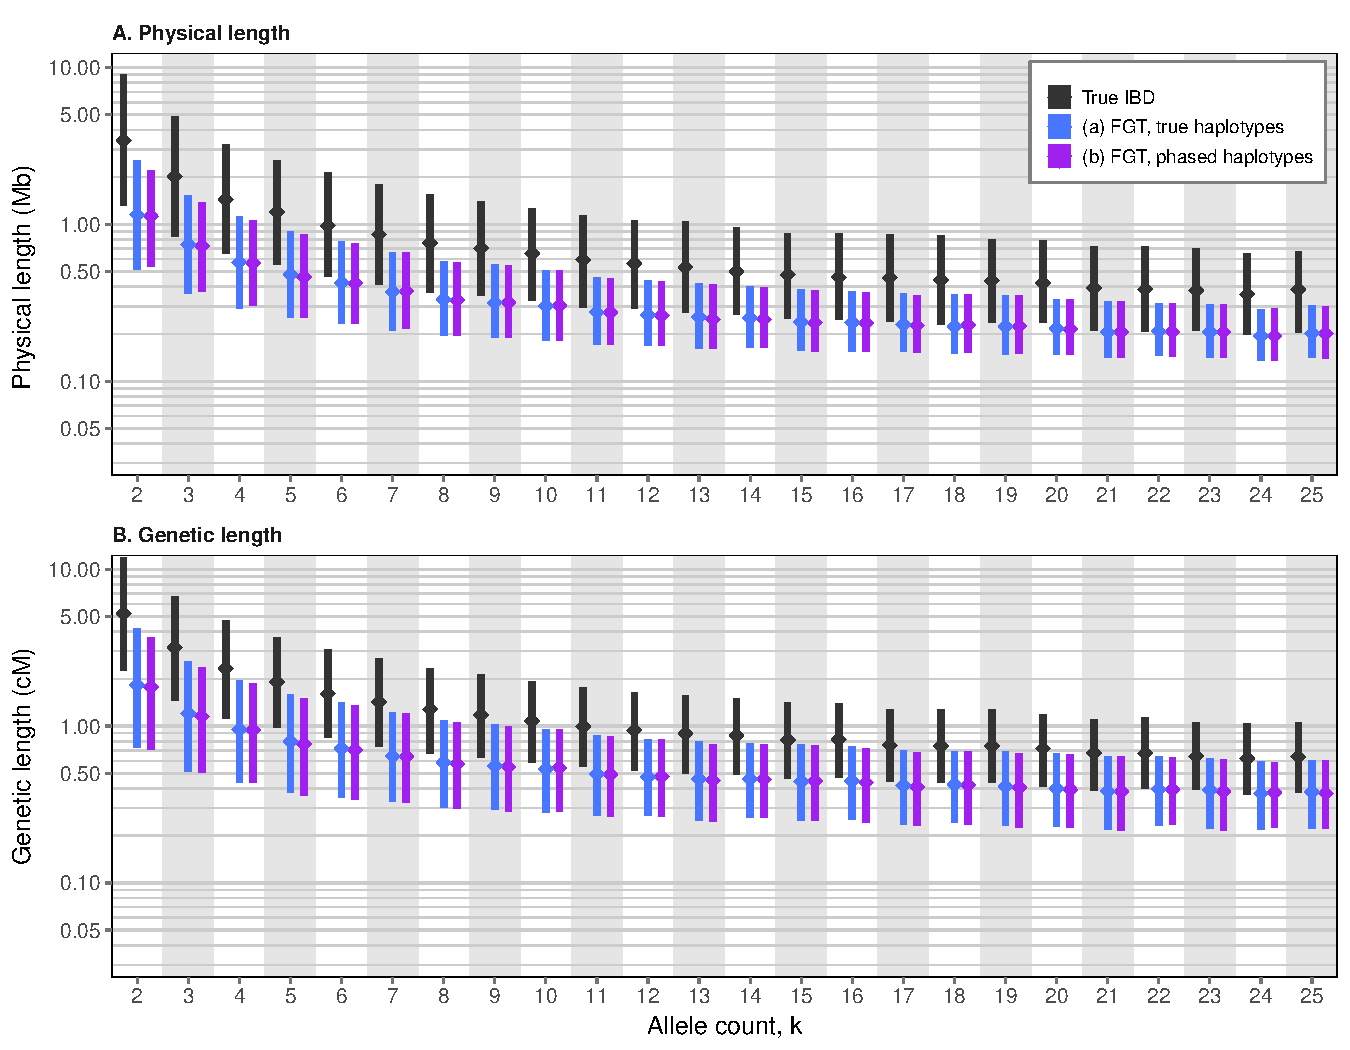
\includegraphics[width=\textwidth]{./img/ch3/beagle_length_tru}
\Caption{IBD segment lengths inferred using \emph{Refined\,IBD} in Beagle~4.1}
{The distribution of median physical and genetic segment length is shown by allele count (\fk{}~category).
IBD segments were estimated using the \texttt{Refined\,IBD} algorithm implemented in \texttt{Beagle~4.1}.
Because the method requires haplotype data, only the \gls{fgt} was evaluated using true haplotypes, \cref{app:fgt_h}, and phased haplotypes, \cref{app:fgt_p}.
These are compared to the true lengths of corresponding IBD tracts.
Bottom and top of each bar indicate \nth{1} and \nth{3} quartiles, respectively, between which the median (\nth{2} quartile) is marked (\emph{diamonds}).}
{fig:beagle_length_tru}
\end{figure}
